\documentclass[14pt]{extbook}
\usepackage{multicol, enumerate, enumitem, hyperref, color, soul, setspace, parskip, fancyhdr} %General Packages
\usepackage{amssymb, amsthm, amsmath, bbm, latexsym, units, mathtools} %Math Packages
\everymath{\displaystyle} %All math in Display Style
% Packages with additional options
\usepackage[headsep=0.5cm,headheight=12pt, left=1 in,right= 1 in,top= 1 in,bottom= 1 in]{geometry}
\usepackage[usenames,dvipsnames]{xcolor}
\usepackage{dashrule}  % Package to use the command below to create lines between items
\newcommand{\litem}[1]{\item#1\hspace*{-1cm}\rule{\textwidth}{0.4pt}}
\pagestyle{fancy}
\lhead{Progress Quiz 8}
\chead{}
\rhead{Version B}
\lfoot{4553-3922}
\cfoot{}
\rfoot{Fall 2020}
\begin{document}

\begin{enumerate}
\litem{
Write the equation of the line in the graph below in Standard form $Ax+By=C$. Then, choose the intervals that contain $A, B, \text{ and } C$.
\begin{center}
    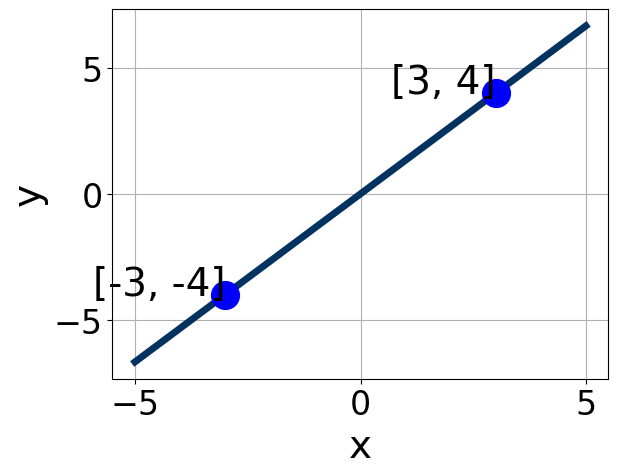
\includegraphics[width=0.5\textwidth]{../Figures/linearGraphToStandardB.png}
\end{center}
\begin{enumerate}[label=\Alph*.]
\item \( A \in [-4.67, 2.33], \hspace{3mm} B \in [-1.4, -0.58], \text{ and } \hspace{3mm} C \in [-1.82, -0.53] \)
\item \( A \in [5, 9], \hspace{3mm} B \in [-3.46, -2.21], \text{ and } \hspace{3mm} C \in [-3.33, -2.68] \)
\item \( A \in [5, 9], \hspace{3mm} B \in [1.87, 4.09], \text{ and } \hspace{3mm} C \in [1.53, 3.37] \)
\item \( A \in [-6, -4], \hspace{3mm} B \in [1.87, 4.09], \text{ and } \hspace{3mm} C \in [1.53, 3.37] \)
\item \( A \in [-4.67, 2.33], \hspace{3mm} B \in [0.29, 2.29], \text{ and } \hspace{3mm} C \in [-0.08, 1.04] \)

\end{enumerate} }
\litem{
Solve the equation below. Then, choose the interval that contains the solution.\[ -11(-3x + 8) = -16(2x -9) \]\begin{enumerate}[label=\Alph*.]
\item \( x \in [-0.2, 1.7] \)
\item \( x \in [-57, -54.4] \)
\item \( x \in [2.2, 3.9] \)
\item \( x \in [-1.7, 0.5] \)
\item \( \text{There are no real solutions.} \)

\end{enumerate} }
\litem{
Solve the linear equation below. Then, choose the interval that contains the solution.\[ \frac{-9x -6}{5} - \frac{-3x -7}{8} = \frac{-9x + 7}{6} \]\begin{enumerate}[label=\Alph*.]
\item \( x \in [18.89, 21.89] \)
\item \( x \in [42.22, 46.22] \)
\item \( x \in [-2.5, 1.5] \)
\item \( x \in [80, 83] \)
\item \( \text{There are no real solutions.} \)

\end{enumerate} }
\litem{
Find the equation of the line described below. Write the linear equation as $ y=mx+b $ and choose the intervals that contain $m$ and $b$.\[ \text{Perpendicular to } 7 x - 6 y = 15 \text{ and passing through the point } (-6, -5). \]\begin{enumerate}[label=\Alph*.]
\item \( m \in [-1.11, -0.76] \hspace*{3mm} b \in [0.98, 1.65] \)
\item \( m \in [-1.11, -0.76] \hspace*{3mm} b \in [9.36, 11.16] \)
\item \( m \in [-1.37, -1.02] \hspace*{3mm} b \in [-11.03, -9.97] \)
\item \( m \in [-1.11, -0.76] \hspace*{3mm} b \in [-11.03, -9.97] \)
\item \( m \in [0.68, 1.49] \hspace*{3mm} b \in [-0.81, 0.79] \)

\end{enumerate} }
\litem{
First, find the equation of the line containing the two points below. Then, write the equation as $ y=mx+b $ and choose the intervals that contain $m$ and $b$.\[ (6, -4) \text{ and } (-2, -7) \]\begin{enumerate}[label=\Alph*.]
\item \( m \in [-0.2, 3.8] \hspace*{3mm} b \in [5.61, 7.1] \)
\item \( m \in [-0.2, 3.8] \hspace*{3mm} b \in [-6.9, -5.43] \)
\item \( m \in [-0.2, 3.8] \hspace*{3mm} b \in [-11.84, -9.25] \)
\item \( m \in [-0.2, 3.8] \hspace*{3mm} b \in [-5.43, -4.92] \)
\item \( m \in [-1, 0.2] \hspace*{3mm} b \in [-8.76, -7.56] \)

\end{enumerate} }
\litem{
Solve the linear equation below. Then, choose the interval that contains the solution.\[ \frac{-9x + 4}{5} - \frac{-4x -5}{6} = \frac{-7x + 5}{7} \]\begin{enumerate}[label=\Alph*.]
\item \( x \in [5.89, 9.89] \)
\item \( x \in [-2.46, 4.54] \)
\item \( x \in [30, 32] \)
\item \( x \in [-6.61, -3.61] \)
\item \( \text{There are no real solutions.} \)

\end{enumerate} }
\litem{
Find the equation of the line described below. Write the linear equation as $ y=mx+b $ and choose the intervals that contain $m$ and $b$.\[ \text{Parallel to } 6 x - 7 y = 6 \text{ and passing through the point } (5, 3). \]\begin{enumerate}[label=\Alph*.]
\item \( m \in [0.74, 0.88] \hspace*{3mm} b \in [-1.3, 0] \)
\item \( m \in [-1.19, -0.74] \hspace*{3mm} b \in [5.4, 8.3] \)
\item \( m \in [0.74, 0.88] \hspace*{3mm} b \in [-2.6, -1.8] \)
\item \( m \in [0.74, 0.88] \hspace*{3mm} b \in [0.4, 4.4] \)
\item \( m \in [0.86, 1.32] \hspace*{3mm} b \in [-1.3, 0] \)

\end{enumerate} }
\litem{
Solve the equation below. Then, choose the interval that contains the solution.\[ -10(-8x + 19) = -3(7x + 5) \]\begin{enumerate}[label=\Alph*.]
\item \( x \in [1.64, 1.84] \)
\item \( x \in [1.92, 2.14] \)
\item \( x \in [-2.24, -1.98] \)
\item \( x \in [3.28, 3.51] \)
\item \( \text{There are no real solutions.} \)

\end{enumerate} }
\litem{
First, find the equation of the line containing the two points below. Then, write the equation as $ y=mx+b $ and choose the intervals that contain $m$ and $b$.\[ (5, 7) \text{ and } (6, 5) \]\begin{enumerate}[label=\Alph*.]
\item \( m \in [-4, 1] \hspace*{3mm} b \in [0.6, 2.5] \)
\item \( m \in [-4, 1] \hspace*{3mm} b \in [-18.7, -16] \)
\item \( m \in [-4, 1] \hspace*{3mm} b \in [-3.3, 0.8] \)
\item \( m \in [-1, 10] \hspace*{3mm} b \in [-7.8, -5.1] \)
\item \( m \in [-4, 1] \hspace*{3mm} b \in [16.7, 19.1] \)

\end{enumerate} }
\litem{
Write the equation of the line in the graph below in Standard form $Ax+By=C$. Then, choose the intervals that contain $A, B, \text{ and } C$.
\begin{center}
    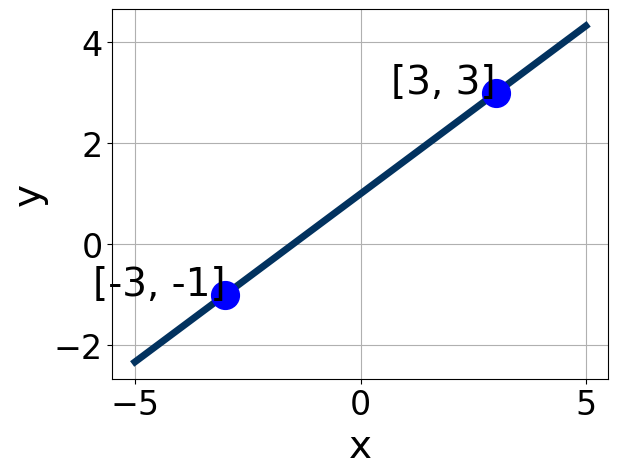
\includegraphics[width=0.5\textwidth]{../Figures/linearGraphToStandardCopyB.png}
\end{center}
\begin{enumerate}[label=\Alph*.]
\item \( A \in [-5, -2], \hspace{3mm} B \in [-5.49, -3.73], \text{ and } \hspace{3mm} C \in [-5.7, -2.9] \)
\item \( A \in [2, 6], \hspace{3mm} B \in [-5.49, -3.73], \text{ and } \hspace{3mm} C \in [-5.7, -2.9] \)
\item \( A \in [-3.2, 3.8], \hspace{3mm} B \in [-1.53, 0.74], \text{ and } \hspace{3mm} C \in [-4.4, 0.8] \)
\item \( A \in [-3.2, 3.8], \hspace{3mm} B \in [0.53, 3.2], \text{ and } \hspace{3mm} C \in [0.6, 1.1] \)
\item \( A \in [2, 6], \hspace{3mm} B \in [3.33, 5.56], \text{ and } \hspace{3mm} C \in [3.6, 6.5] \)

\end{enumerate} }
\end{enumerate}

\end{document}